% 1999 年全国卷理科第 10 题：多面体 ABCDEF
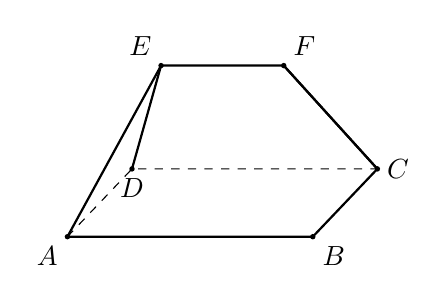
\begin{tikzpicture}[scale=0.82, >=stealth]
  \coordinate (A) at (0,0);
  \coordinate (B) at (3.8,0);
  \coordinate (C) at (4.8,1.05);
  \coordinate (D) at (1.0,1.05);
  \coordinate (E) at (1.45,2.65);
  \coordinate (F) at (3.35,2.65);

  \draw[thick] (A)--(B)--(C)--(F)--(E)--cycle;
  \draw[thick] (F)--(C);
  \draw[dashed] (A)--(D)--(C) (D)--(E);
  \draw[thick] (D)--(E);

  \fill (A) circle (1.2pt) node[below left] {$A$};
  \fill (B) circle (1.2pt) node[below right] {$B$};
  \fill (C) circle (1.2pt) node[right] {$C$};
  \fill (D) circle (1.2pt) node[below] {$D$};
  \fill (E) circle (1.2pt) node[above left] {$E$};
  \fill (F) circle (1.2pt) node[above right] {$F$};
\end{tikzpicture}
